\documentclass[aps,pra,twocolumn,groupedaddress,showpacs]{revtex4}

\usepackage[latin1]{inputenc}
\usepackage[T1]{fontenc}
\usepackage{amsmath,amssymb}
\usepackage{bbm}
\usepackage{graphicx}
\usepackage{subfigure}
\usepackage{sistyle}
\usepackage{ifpdf}
\usepackage{xcolor}
\usepackage{physics}



\begin{document}

\title{Quantum estimation of a fluctuating perturbation}

\author{Claus Normann Madsen}
\author{Lia Valdetaro}
\author{Klaus M\o lmer}
\affiliation{Department of Physics and Astronomy, University of Aarhus, DK-8000 Aarhus C, Denmark}


\begin{abstract}

This article describes the estimation of a fluctuating physical quantity that acts as a perturbation on a continuously monitored quantum system. The theory combines a Hidden Markov Model and quantum measurement theory into a time evolving hybrid classical and quantum trajectory. The classical forward-backward theory that permits smoothed estimates of Hidden Markov Models has a counterpart in the theory of quantum trajectories and past quantum states. We present examples of application of this theory and show how it improves parameter estimation.


\end{abstract}

\maketitle

\section{Introduction}

The use of quantum systems for precision measurements is one of the emerging so-called quantum technologies that is already offering benefits to society. Atomic systems are ideal time keepers, and they are sensitive over broad band widths to perturbations such as magnetic and electric fields. A host of quantum features are being employed from squeezing, to exploitation of entanglement, quantum error correction  and phase transitions to achieve the maximum measurement sensitivity. Measurement outcomes are governed by Borns rule and a fundamental randomness, which play important roles for the precision and sensitivity of any metrological protocol. In case of continuous measurements over time, the randomness is accompanied by measurement back action, which quenches the quantum system and affects subsequent measurements. This may yield higher sensitivity to perturbations than one would infer from their influence on the deterministic evolution of mean values.

In this article we employ quantum trajectory theory, i.e., stochastic master equations that describe the evolution of a system density matrix conditioned on both the unitary and dissipative evolution of the system and on the random outcomes of measurements on the system. We incorporate an unknown classical perturbation by a Hidden Markov Model (HMM)CITE  with hidden states $n$ among which jumps occur with rates $r_{n\rightarrow m}$, and which govern the dynamics of the quantum system, e.g., through the value of terms in the system Hamiltonian. Measurements on the system serve to probe its evolution and may reveal the strength or other properties of the perturbation on the system. The hidden states may in the most general case control any aspect of the quantum dynamics, coherent coupling rates, incoherent coupling strengths, and even fundamentally different types of evolution as represented by entirely different terms in the system master equation. As a less speculative  example we study here the case of a fluctuating magnetic field which causes fluctuations in the transition frequency of a resonantly driven transition in a two-level system in an optical cavity, and we use the noisy outcome of homodyne detection of the signal emitted by this system to estimate the time dependent detuning, i.e., magnetic field. Following work by Belavkin CITE, we extend the quantum state formalism to incorporate the unknown classical variable $n$ as if it was a an additional effective quantum degree of freedom, absent of coherences and with populations that are subject to the rate equations of the HMM. The back action of measurements on the quantum system act on the full density matrix on the combined system Hilbert space and classical parameter space, and effectively yields a Bayesian updates of our knowledge of the fluctuating parameter. The same theory extends to the use of full measurement records to determine outcome probabilities and hence the most likely outcome values of past measurements on the system CITE PQS. When applied to the unknown classical perturbation, this constitutes our best estimate of its time evolution.

The article is organized as follows. In Sec. II, we present our physical sensing device composed of a two-level spin system in a cavity which is driven by a classical field. We eliminate the cavity field and present the stochastic master equation for the two-level system subject to continuous homodyne detection of the cavity output field. In Sec III, we introduce the joint stochastic master equation describing the conditional classical and quantum dynamics of the HMM and the probe quantum system, and we provide the explicit theory for the case of the fluctuating magnetic field and the two level system subject to homodyne detection. In Sec. IV we recall the past quantum state formalism and we discuss how it generally leads to the time dependent probability distribution of the HMM variable govering the dynamics of the quantum system. We provide explicit theory and simulations in case of homodyne detection, conditioned on the entire homodyne measurement record.  Sec. V concludes and presents an outlook.

\section{Description of the model}

\subsection{A resonantly driven spin system}

Following CITE HaikkaBertet we consider the situation of a two-level system in a cavity subject to a classical driving field at the frequency $\omega_d$. The reflected signal is subject to homodyne detection and will thus reveal the interaction of the two-level system with a time dependent magnetic field that shifts its resonance frequency with respect to the one of the cavity and the classical drive field.   

The monitored system consists of a two-level atom in a cavity, and it is monitored by homodyne detection. The cavity is damped faster than the other dynamical time scales, and the cavity field degrees of freedom can therefore be adiabatically eliminated. In a frame rotating with the driving field, $\beta_{in} = \beta e^{i\omega_d t}$, the Hamiltonian of the qubit and cavity can be written as
\begin{equation}
H = \Delta_r \hat a^\dag \hat a + i \sqrt{2\kappa_1} (\beta \hat a^\dag - \beta ^* \hat a) + \frac{\Delta_s}{2} \hat \sigma_z + g(\hat \sigma_+ \hat a + \hat \sigma_- \hat a^\dag), \label{initial_Hamiltonian}
\end{equation}
where $\Delta_r$ is the detuning between the driving field and the cavity, $\hat a$ ($\hat a ^\dag$) is the annihilation (creation) operator of the photonic field in the cavity,
$\kappa_1$ is the amplitude decay rate of the cavity field due to transmission to the outgoing field, $\beta$ is the amplitude of the driving field. The atom or spin system is characterized by the $\hat \sigma_z$  and $\hat \sigma_+$ ($\hat \sigma_-$) Pauli-$Z$ and raising (lowering) operators, the detuning $\Delta_s$ between the qubit spin and the driving field, and the coupling strength $g$ with the quantized cavity field.

The system is subject to damping processes represented by Lindblad operators 
\begin{align}
\hat c_1 =& \sqrt{2\kappa} \hat a \\
\hat c_2 =& \sqrt{\gamma_{dec}} \hat \sigma_- \label{c2}\\
\hat c_3 =& \sqrt{\frac{\gamma_\phi}{2}} \hat \sigma_z. \label{c3}
\end{align}
Here, $\hat c_1$ is the decay of the photon field in the cavity either by transmission (rate $\kappa_1$) or losses (rate $\kappa_L$, $\kappa=\kappa_1+\kappa_L$). $\hat c_2$ denotes the possible decay of the qubit excitation outside of the cavity mode, and $\hat c_3$ denotes dephasing of the qubit.

The outgoing field from the cavity is given by input-output theory 
\begin{equation}
\hat c_{out} = \sqrt{2\kappa_1}\hat a - \beta,
\end{equation}
the homodyne detection of the outgoing  field causes measurement back action and is represented by a stochastic term in the master equation involving the operator $\hat c_{out}$. 

\subsubsection{Adiabatic elimination of the bad cavity}

The cavity facilitates efficient probing of the spin system, but in the bad cavity limit $g \ll \kappa$, the cavity degrees of freedom follow the evolution of the spin closely, and the may be adiabatically eliminated from the formalism.
This considerably simplifies the system of equations.


The cavity field operator $\hat a$ obeys the Heisenberg equation of motion,
\begin{equation}
\pdv{\hat a}{t} = - i \Delta_r \hat a + \sqrt{2\kappa_1}\beta - ig \hat \sigma_- - \kappa \hat a + \hat F,
\end{equation}
where $\hat F$ is the input vacuum field Langevin noise with vanishing expectation value. Omitting the noise and setting $\pdv{\hat a}{t}=0$, permits ellimination of $\hat a$ under the assumption of adiabatic following of the qubit in the frame rotating with frequency $\omega_s$,
\begin{equation}
\hat a = \frac{\sqrt{2\kappa_1}\beta}{\kappa + i \Delta_r} - \frac{i g \hat \sigma_-}{\kappa + i (\Delta_r - \Delta_s)}.
\end{equation}
Inserting this expression in \eqref{initial_Hamiltonian} and \eqref{c3} we obtain the effective qubit Hamiltonian
\begin{equation} \label{Hadel}
H = \frac{\Delta_s}{2} \hat \sigma_z + g(\alpha \hat \sigma_+ + \alpha^* \hat \sigma_-) - \epsilon_s \hat \sigma_+ \hat \sigma_-,
\end{equation}
where $\alpha=\frac{\sqrt{2\kappa_1}\beta}{\kappa + i \Delta_r}$ and $\epsilon_s = \frac{g^2 (\Delta_r - \Delta_s)}{\kappa^2 + (\Delta_r - \Delta_s)^2}$, and 
\begin{equation}
\hat c_1 = \sqrt{\gamma_p}\hat \sigma_-, \label{c1}
\end{equation}
with the Purcell-enhanced decay rate
\begin{equation}
\gamma_p = \frac{2 g^2 \kappa}{\kappa^2 + \left(\Delta_r - \Delta_s\right)^2}.
\end{equation}

Finally, the out-coupled field is conveniently represented by the operator
\begin{equation}
\hat c_{out} =  \sqrt{2\kappa_1}\left( \alpha - \frac{i g \hat \sigma_-}{\kappa + i (\Delta_r - \Delta_s)} \right) - \beta \label{cout}
\end{equation}

\subsubsection{Homodyne measurement master equation}
A quantum system subject to homodyne detection evolves according to the stochastic master equation (SME) $\tilde\rho(t+dt)= \tilde\rho(t) + d\tilde\rho$ where 
\begin{equation}
d\tilde \rho = \mathcal{L} \tilde \rho dt + \mathcal{X}_\Phi \tilde \rho dY_t, \label{forward_homodyne_master_equation}
\end{equation}
where the tilde indicates that the evolution is not normalized. The first term yields the usual Lindbad master equation terms
\begin{equation} \label{LME}
\mathcal{L}\rho = -i\comm{\hat H}{\rho} + \sum_i\mathcal{D}[\hat c_i]\rho,
\end{equation}
where $H$ and $\hat c_i$ are the Hamiltonian and Lindblad damping operators presented in the previous subsection with $\mathcal{D}[\hat A] \rho = 	\hat A \rho \hat A^\dag - \frac{1}{2} (\hat A^\dag \hat A\rho + \rho\hat A^\dag \hat A)$. The second term in \eqref{forward_homodyne_master_equation} $\mathcal{X}_\Phi dY_t$ represents the back action due to the homodyne measurement of the output field, where
\begin{equation}
\mathcal{X}_\Phi \rho = \sqrt{\eta} \left(\hat c_{out} e^{-i \Phi} \rho + \rho \hat c_{out}^\dag e^{i \Phi} \right),
\end{equation}
where $\Phi$ is the phase of the local oscillator used for homodyne detection, $\eta$ is the measurement efficiency. $dY_t$ is the measured homodyne signal in the time-step $dt$, and is composed of a mean and a fluctuating contribution,
\begin{equation}
dY_t = \Tr[ \mathcal{X}_\Phi \rho(t) ] dt + dW_t,
\end{equation}
where $dW_t$ is a Wiener increment of zero mean and variance $dt$. The mean values is governed by the expectation value of the $\mathcal{X}_\Phi$ operator with the (normalized) density matrix $\rho^(t)$.

\section{Hybrid classical and quantum description of the unknown perturbation and the quantum probe}
  
\subsection{Hidden markov model of the perturbation}

Hidden Markov Models are powerful tools to analyze time series of data ranging from the natural sciences to linguistics and sociology. In classical applications, the model describes a hidden parameter that explores a discrete space of values (states) by randomly jumping with rates $r_{n\rightarrow m}$ among them. The assumption is that the hidden parameter governs the evolution of the system of interest and that observation of some of its degrees of freedom gives rise to a detection signal with statistics that depends on the state occupied by the Hidden Markov parameter. The change of character over time of the observed signal can thus be ascribed to the changes of this state, and if the probability of a given signal outcome is known for each state, Bayes rule, together with the rate equations, permits evaluation of the probability that the system occupies the different states conditioned on the measurement. Such models show a rich variety of behaviors and both the signal probabilities, the transition rates -  and even the number of states - can be treated as fitting parameters to develop efficient models for various kinds of signals.

We have previously used the HMM to describe incoherent dynamics in quantum physics, such as off resonant excitation and spontaneous decay causing transfer between hyperfine atomic states with different excitation frequencies monitored by cavity transmission probing CITE GammelmarkMeschedeArticle and the fluctuations of the photon number in a microwave cavity subject to quantum non-demolition dispersive interaction with a sequence of probe atoms CITE DotsenkoHaroche. In this article our aim is to employ the hidden markov model to represent an unknown time dependent physical perturbation. While our treatment is general, we shall study the example of a hidden markov model which corresponds to a discrete version of the stochastic Ornstein-Uhlenbeck process, a diffusion process with a long time steady state  Gaussian distribution. This discrete model is also known as the Ehrenfest dog-flea model, describing the evolution of the difference in the number of randomly jumping fleas between two dogs.

In our example, the discrete variable $n$ represents the fluctuating candidate value $B_n$ of a magnetic field, which causes an energy shift of a spin eigenstate or an atomic Zeeeman sub-level and hence a variation of the detuning $\Delta_s$ in the model described in the previous section. We add this perturbation to the model after the adiabatic elimination, and we only consider its immediate effect on the first term $\frac{\Delta_s}{2} \hat \sigma_z$ in \label{Hadel} while the minor influence on the coefficent $\epsilon_s$ is omitted in the following.

\subsubsection{Extending the density matrix to include the fluctuating perturbation}

A joint classical quantum description of the system makes use of the fact that the HMM is equivalent to the dynamics of a quantum system restricted to populate the states $n$ incoherently. In such a description the transitions between the states can be represented by quantum jump Lindblad terms
\begin{equation}
\hat J_{nn'} = \sqrt{r_{nn'}} \dyad{n'}{n} \label{Linblad_B_Jump_Operator}
\end{equation}
acting on the classical state components of a two-component density matrix on the extended Hilbert space
\begin{eqnarray} \label{block}
\tilde{\rho} = \sum_n \tilde{\rho}_n \otimes \dyad{n}{n}\nonumber \\
\begin{bmatrix}
\tilde{\rho}_1 & & & 0\\
& \tilde{\rho}_2 & & \\
& & \ddots & \\
0 & & & \tilde{\rho}_N
	\end{bmatrix}.
\end{eqnarray}
Each $\tilde{\rho}_n$ term is an unormalized density matrix on the Hilbert space of the two-level system, correlated with the diagonal elements $\dyad{n}{n}$, i.e., with the unknown classical value $B_n$ of the magnetic field. We emphasize that the unknown perturbation is now treated in complete equivalence with an additional quantum degree of freedom of an enlarged system. The full density matrix of that system solves the stochastic master equation \eqref{LME}, where in addition to the terms acting on each $\tilde{\rho}_n$ component (note that $c_i \rightarrow c_i \otimes \sum_n \dyad{n}{n}$, and the Hamiltonian $H= \sum_n H_n\otimes \dyad{n}{n}$ depends on $n$ through the detuning parameter in CITE EQ), the system is subject to Lindblad like terms, $\sum_{nn'}\mathcal{D}[I\otimes\hat J_{nn'}]\rho$ which distribute the atomic system density matrix elements among the sub-blocks in \eqref{block} to represent the probabilistic evolution of the hidden parameter (the magnetic field).

Normalizing $\tilde{\rho}$ to unit trace, is equivalent to the scaling of all $\rho_{n}=\tilde{\rho}_n/Tr(\tilde{\rho})$, which yields the probability distribution of the magnetic field as the population of the corresponding hidden state $n$, $P(B_n)=Tr(\rho_n$. 

The dynamics of the full system density matrix \eqref{block}, subject to the various elements of the master equation, and in particular to the measurement back action, is a direct implementation of the Belavkin filter idea CITE. The redistribution of probability among the candidate values $B_nb$ is equivalent to a Bayesian update, since the change in norm of each $\tilde{\rho}_n$ due to the term in \eqref{LME} proportional to the measurement outcome $dY_t$ directly represents the probabilty of that outcome conditioned on the state. The trace of the $\tilde{\rho}_n$ components that are most compatible with the outcome thus experience a relative increase, as classically evolving HMM state probabilities are similarly favored by the measurement signals most compatible with their statistics. In the quantum filter version, this theory was so far mostly applied to either specific systems with Gaussian distributions or to the estimation of constant parameters.

\subsection{Specification of system for sensing of magnetic field} 

Subjecting the system to a magnetic field $B_z(t)$ changes the qubit energy difference through the Zeeman effect,
\begin{equation}
H_{Z} = -\frac{g\mu}{2}B_z(t) \hat \sigma_z,
\end{equation}
where $g$ is the Lande factor and $\mu$ is the electron magnetic moment.  

For a range of discrete values $B_n$ of the magnetic field, the system Hamiltonian thus attains the values
\begin{equation}
\hat H_{n} = \frac{\Delta_s(B_n)}{2}\hat \sigma_z + g \left(\alpha \hat \sigma_+ + \alpha^* \hat \sigma_-\right) - \epsilon_s(i) \hat \sigma_+ \hat \sigma_-,
\end{equation}
where
\begin{equation}
\Delta_s(B_n) = \Delta_s - \frac{g_{q_B} \mu}{2} B_n.
\end{equation}

We could assume any HMM represnetation of a flcurtuating magnetic field, but we choose a mode that mimics the Ornstein-Uhlenbeck diffusion like process with jumps only between neighbouring values of the B-field during time steps that have to be sufficiently small that multiple jumps can be disregarded. See CITE: "Of Dogs and Fleas: The Dynamics of N Uncoupled Two-State Systems" by Ch. Hauert, J. Nagler, and H. G. Schuster, Editor, Year City. 

\subsection{Numerical example}

KLAUS: Something about the parameters, the size of the n-grid , the dog flea parametrization and the drive strength of the probe field. Fine to switch to detuning instead of B field. but we should still elaborate a little on the chosen parameters.

% CLAUS: Below section on parameters and n-grid size added. 7/2/2021
In the simulations, we use natural units of $\hbar = 1$ and rescale all parameters in terms of a characteristical time scale, $\gamma$. In terms of these units, the single-photon coupling strength $g = 2 \gamma$ and the cavity field decay rates $\kappa = \kappa_1 = 10 \gamma$. The driving laser and the cavity are assumed to be in resonance, $\Delta_c = 0$. The characteristic time scale $\gamma$ is chosen to be equal to the free decay rate of the qubit, $\gamma = \gamma_{dec}$, and the qubit dephasing rate is matched to this value $\gamma_\Phi$, giving competing sources of noise. The space of detuning-values probed is $\Delta_n \in [2,..,-2] \gamma$.


This choice of parameters leads to a cavity-qubit detuning-dependent (and thus magnetic field dependent) Purcell-enhanced spontaneous decay rate between $\gamma_p(\Delta_n = 0) = \frac{4}{5} \gamma$ for the central value of the magnetic field and $\gamma_p(\Delta_n = \pm 2) = \frac{10}{13} \gamma$ at the extremes of our estimation grid. Thus, the process of the qubit decaying by pumping the cavity field with a photon is much slower than the cavity field decay rate, as demanded by the adiabatic elimination of the cavity state-space. We chose the strength of the coherent drive to be $\beta = 3\sqrt{\gamma}$ and thus also much faster than the enhanced qubit decay into the cavity.


The simplified dog-flea model which we implemented as our example HMM is parametrized only by a base jump rate, corresponding to the rate at which a single flea jumps independently of other fleas, and the total number of fleas in the two-dog system. In our example system, the base jump rate $p$ is simply a characteristic scale of magnetic field changes and the total number of fleas $N$ translates to the number of discrete magnetic field states included in the HMM. For a given choice of $p$, the dog-flea model state parameter probability distribution tends to the Ornstein-Uhlenbeck process with infinitesimal parameters $\mu = N/2$, $\theta = 2 p$ and $\sigma = \sqrt{pN}$ for large $N$. For our simulations, we chose a state space of size $N=25$, corresponding to a dog-flea model with $24$ fleas, and a basis rate of $p = 0.02\gamma$. The maximum field jump rate is then $12 p = 0.24\gamma$, or just under $\frac{1}{4} (\gamma t)^{-1}$.


With such parameters we have simulated the time dependent magnetic field $B(t)=B_{n(t)}$ and used it to drive the quanum system by the Hamiltonian $H_{n(t)}$. A typical homodyne detection record was subsequently constructed by parallel propagation of the stochastic master equation of the small system \eqref{SME} and  simulation of the $dW$ white noise term in the expression for $dY_t$ CITEREF. Fig.1 shows the true magnetic field as a red curve. The simulated current is fed to our master equation for the extended density matrix \eqref{block}, and $P(B_n,t)=$Tr($\rho_n(t)$) is evaluated from the renormalized density matrix. The bright colored region in Fig.1 shows the timedependent region with the highest conditional probability and is in good agreement with the actual simultade value. The green curve shows the maximum likelihood value. It generally follows the exact value well, while it is unable to immediatley follow rapd changes and it generally lags behind the true value. This is no surprise, since the homodyne detection is a noisy process and thus requires integration over time to yield significant informsation, and the qubit probe is itself a damped resonator wiht a finite bandwidth and response time to the external pertubation.

 \begin{figure}[h!]
    \centering
    \centering
    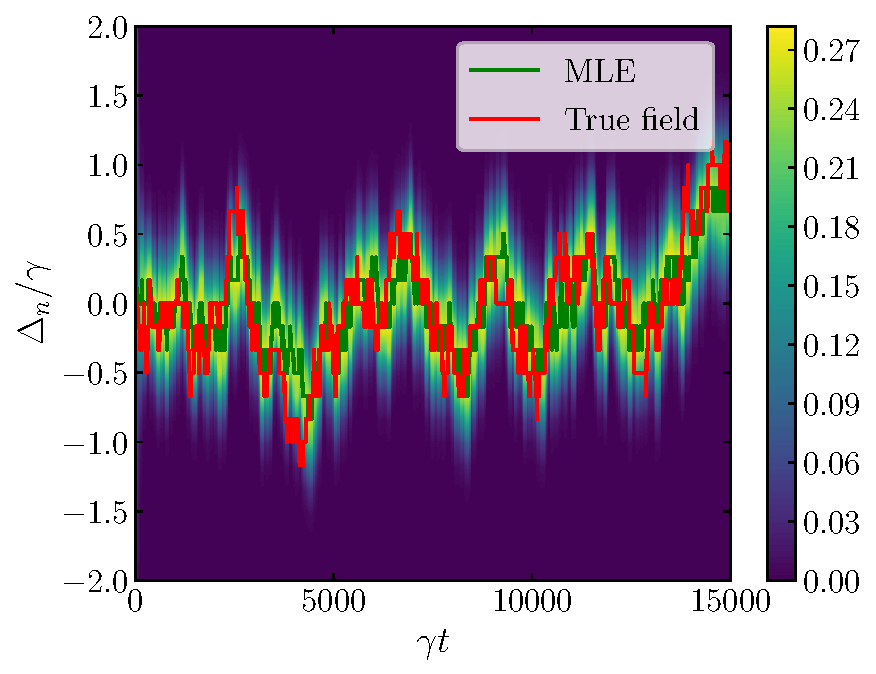
\includegraphics[width=0.4\textwidth]{filtering.pdf}
    \caption{Conditional probability distribution for the time dependent magnetic field acting on the qubit system. }
\end{figure}

KLAUS: Something about the results.  The width averaged through time is 0.32 and the mean error is 0.33 something about units and the other parameters. 


\section{Forward-backward estimate by the Past Quantum State formalism}
The Hidden Markov Models permit estimation of the hidden parameter by a Bayesian update mechanism, expressing the conditional probability of the current state in terms of the joint probability of the state {\it and} all previous signal outcomes. As future measurement statistics are similarly governed by the state, the probability distribution of the state at time $t$ is also correlated with the measurement outcomes {\it after} $t$. The Markovian assumption permits resolution of these correlations and identification of recursive equations, one propagating the probability of the state at time $t$ forward in time conditioned on previous signal data, the other propagating backwards towards earlier times the probability of the actually measured  subsequent data conditioned on the state at time $t'$ . Multiplication of these two state dependent functions at the same time $t$ yields the smoothed estimate, which is nothing but the joint probability for the signal at all times and the state at time $t$,  evaluated at all the known data CITE Gammelmark,NUMREC.

A similar concept applies to the state of a monitored quantum system, where instead of assigning probabilities to classically occupied quantum states, we assign probabilities to outcomes of particular measurements at time $t$ during a longer probing sequence. While the probing may for example be homdyne dtection of an emitted light signal from an atom, these particular measurements may be projective measurements in a certain eigenbasis of the same atom, in which case we may refer to their outcome probabilities, conditioned on homodyne signal as the inferred population of the given state. We caution, however, to generally assign definite  physically occupied state to such a probabilistic assignment, cf, the resulting inconsistency with the outcome probabilities for measurements of complementary observables   CITE MurchMixture. For our purpose, the assignment of probabilities to the classical states $n$ of the HMM is free of such inconsistencies.

In brief, the past quantum state idea is that the stochastic master equations can be understood by writing the quantum trajectory condtional dynamics as  deterministic evolution intercepted by stochastic elements which can in turn be written as POVM operators acting on the state. The probability of a long measurement sequence is then simply given by the trace of an expression that concatenates all these elements, including any particular measurement at any time $t$. If the probing of the system only proceeds until time $t$, the concatenated action of the deterministic evolution and all the probe outcomes is nothing but the conditonal density matrix $\rho(t)$, and we recover the conventional expression for the outcome probability of the 'particular' measurement. If later probing outcomes are condidered, the cyclic properties of the trace permits combination of the corresponding POVM and time evolution in a single matrix $E(t)$, conditioned on only the probing outcomes after $t$. The resulting expression for the outcome probability of an arbitrary measurement with POVM operators $\Omega_m$, reads
\begin{equation} \label{pqsprob}
P(m)=\frac{Tr(\Omega_m \rho(t)\Omega_m^{\dag} E(t))}
{\sum_m' Tr(\Omega_{m'} \rho(t)\Omega_{m'}^{\dag} E(t))}, 
\end{equation}
in comparison with the conventional $P(m)=Tr(\Omega_m \rho(t)\Omega_m^{\dag})$. 

This formalism is similar to the forward-backward analysis of the HMM, but the matrix character and the fact that $\rho$, $\Omega_m$ and $E$ may not have common eigenstates, leads to some quantative differences with the results of classical HMM.


The effective stochastic master equation for $\rho$ subject to homodyne detection is given in \eqref{SME}, and is equivalent to application of the POVM elements 
\begin{equation}
\hat M_{dY_{t}} = (2\pi dt)^{-\frac{1}{4}}e^{\frac{-dY_t^2}{4dt}}\left( \mathbb{1} -i\hat H dt - \frac{\hat c^\dag \hat c}{2}dt + \hat c dY_t\right),
\end{equation} 
associated with the homdyne signal $dY_t$.  KLAUS: phase factor on the last $\hat{c}$ to match the SME ?
The corresponding equation for $E$ is provided in CITE Gammelmark, and it naturally involves the adjoint operation (from the cyclic transfer of the $\hat{M}_{dY_t}$ within the trace expression for the signal record probability
\begin{equation}
E_{t-dt} = \hat M_{dY_{t-dt}}^\dag E_t \hat M_{dY_{t-dt}}.
\end{equation}
Combining all the elements of the evolution yields the backward, adjoint 'master equation'  $E(t-dt)=E(t) + dE(t)$, where $dE(t)$ is conditioned on the homodyne measurement signal $dY_{t-dt}$, 
\begin{align}
dE =& i\comm{\hat H}{E} + \sum_i \mathcal{D}^\dag[\hat c_i]E \nonumber\\
&+ \sqrt{\eta}\left( \hat c_{out}^\dag E + E\hat c_{out} \right)dY_{t-dt},
\end{align}
KLAUS Phase of local oscillator, 
and $\mathcal{D}^\dag$ denotes the adjoint Linblad term dissipator
\begin{equation} \label{ladj}
	\mathcal{D}^\dag[\hat A] E = \hat A^\dag E \hat A - \frac{1}{2} \acomm{\hat A^\dag \hat A}{E}.
\end{equation}


The incorporation of the classically fluctuating parameter by the HMM, is equivalent to the one for $\rho(t)$, i.e., we introduce the extended block-diagonal operator $E(t)$,
\begin{align} \label{blockE}
E =& \sum_n E(n) \otimes \dyad{n}{n}\nonumber \\
=& \begin{bmatrix}
E_1 & & & 0\\
& E_2 & & \\
& & \ddots & \\
0 & & & E_N
\end{bmatrix},
\end{align}
and its evolution incorporates the conjugate Lindblad terms cf., \eqref{ladj} with $\hat{A}=\hat{J}_{nn'}$. Unlike the forward HMM for which these transitions rates yields a steady state distribution that balances the transitions among the HMM states $n$, the backward adjoint rate equations have the uniform distribution as its steady state, as readily seen by inserting the identiy matrix for $E$ in \eqref{ladj}. In the presence of probing, however, the $E$ matrix is nontrivial and cntributes to the estimate of the HMM parameter.    

\subsubsection{PQS probabilities for the classically fluctuating HMM parameter}

Solving the equations for $\rho(t)$ and $E(t)$ with the specified Hamiltonians, Lindblad operators and stochastic increments, we are in possession of block matrices \eqref{block} and \eqref{blockE}. The probability of the $n^{^th}$ state of the HMM is given by \eqref{pqsprob}, with the projective operator
$\Omega_m = \dyad{n}{n}$, which up to normalization gives the result.    
\begin{align}
P_{PQS}(B_n, t) =& \Tr(\dyad{n}{n} \rho(t) \dyad{n}{n} E(t)) \nonumber\\
=& \Tr(\rho^{(n)}(t) E^{(n)}(t))  \nonumber \\
=& \rho^{(n)}_{gg}(t)E^{(n)}_{gg}(t) + \rho^{(n)}_{ee}(t)E^{(n)}_{ee}(t) \nonumber \\
&+ \rho^{(n)}_{ge}(t)E^{(n)}_{eg}(t) + \rho^{(n)}_{eg}(t)E^{(n)}_{ge}(t) \label{PQS-trace}.
\end{align}
Note that unlike FORWARD EXPRESSION the retrodicted probability depends on both the populations (through the trace) and the coherences in the system density matrix $\rho_n(t)$ and it does not simply factor into a product of terms conditioned on early and later detection outcomes. In general the PQS estimate smoothens the estimate as fluctuations in the signal $dY_t$ contribute with similar effect to either $\rho$ or $E$, and are hence partially suppressed in joint estimates. It also improves the estimate, essentially because it uses twice as much data (time windows both before and after $t$ for the estimate). Normally that would suggest a factor two reduction of the variance of the estimator, but do to the matric character of the expression \eqref{PQS-trace} and the correlations between $n$ and the still unresolved system statesm this factor may be larger CITE Cheng article.   


Figure 2 shows an analysos of the same dat as was used to produce Figure 1. but where we apply the Past Quantum State formalism and \eqref{PQS-trace} to provide the probability distribution and the maximum liklelihood estimator. The figure shows that the conditional probability of the time dependent  value of the classical pertubation is more tight, and the maximum likelihood estimator (green curve) is generally closer to the correct value. In particuar we now observe no appreciable delay between the true value and the estimator. This is similar to the observation in CITE which applied a different multi-time estimator and in CITE Cheng which applies Kalman filter and smoothing to the case where the classical and quantum variables can be described by a Gaussian probability distribution - see also CITE TSang.

\begin{figure}
    \centering
    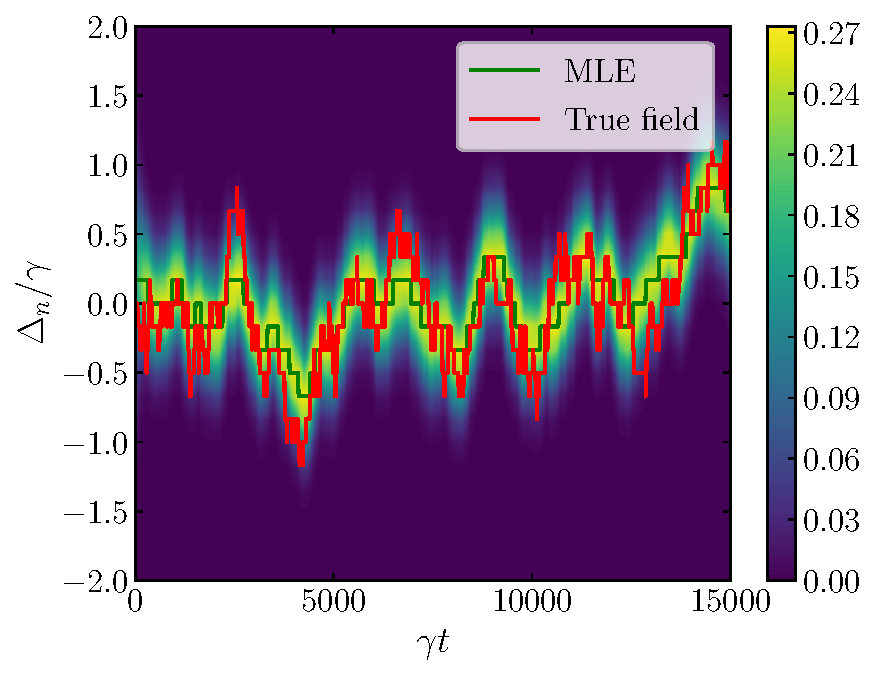
\includegraphics[width=0.4\textwidth]{PQS.pdf}
    \caption{Forward and backward weighted probability distribution. The width averaged through time is 0.26 and the mean error is 0.26.}
\end{figure}
Using both forward and backward weighing of the probabilitiy distribution, as described in the theory section on PQS, the distribution is much smoother through time. The average error between the maximum likelyhood estimator and the true simulated field is much lower at the slow rates chosen for this run for this PQS-propagation than for the forward one. The average width of the distribution is also much lower. Lastly, the maximum likelyhood estimator is not in general lagging behind the true field as it does for the forward propagation due to lag in information gain from the field changing value. Instead, the MLE (maximum likelyhood estimator) is closer to the true field, probably sometimes being slightly ahead and sometimes slightly behind.

KLAUS: I suggest to suppress the next section of the article and just give some numbers for the mean squared erro fo the maximum likelihood estimator. Can we supplement with one or two more cases. For exa,mple with faster and slower noise to see that the quality of the estimators change. For very ast nose, I guess that both estimator would apprioach the unmeasured width of the dog flea model, while their difference is tronger wjhen the noise is slower.


\subsection{Forward and PQS estimator errors vs drive strength}
The two most important characteristics for any estimator are its accuracy and precision. Inspecting both forward and PQS estimation figures from before, it can be seen that on average, the colored regions of higher probability density usually includes the true state. In a true experiment, the experiment would of course not have access to the underlying "true state". We propose however, that the widths of the forward and PQS distributions can be used as measures of the accuracy of the estimator. To show this, the squared mean error of the true state to the weighted mean estimate is compared to the width of the estimator probability distributions in figure \ref{beta_figure}. This figure includes the dependence of all four parameters on the strength of the coherent drive.

 \begin{figure}[h!]
    \centering
    \centering
    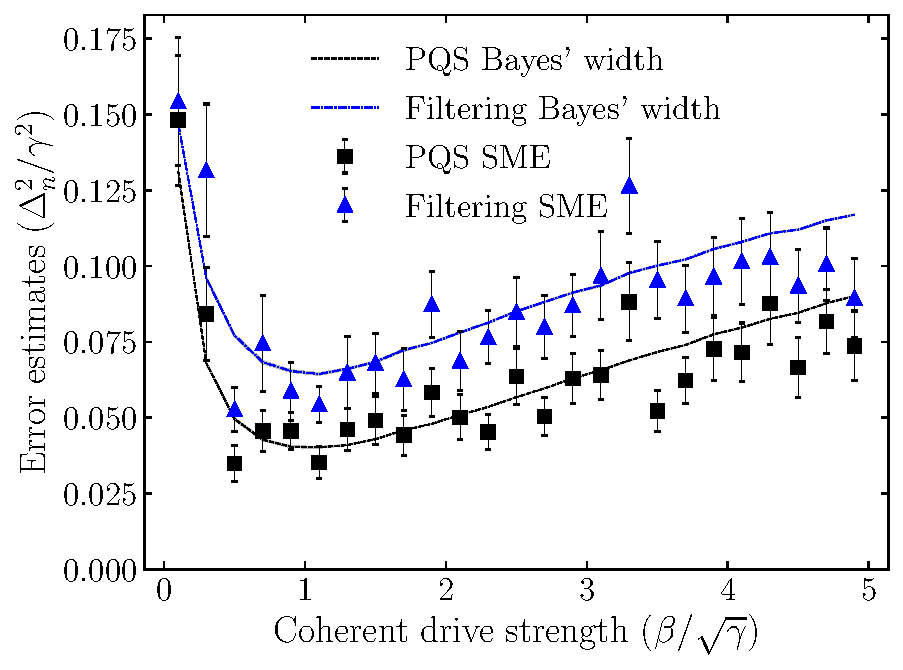
\includegraphics[width=0.4\textwidth]{drive_strength_figure.pdf}
    \caption{Averaged Bayes' widths and squared mean errors of weighted distribution means vs the simulated true states for both the filtering and PQS estimators, as functions of driving strength $\beta$}
    \label{beta_figure}
\end{figure}

Figure \ref{beta_figure} furthermore provides an intuition on how the amount of extracted information depends on the strength of the coherent drive. At too low driving, the qubit is hardly driven and thus doesn't emit information carrying photons. On the other end of the scale, driving too hard leads to power broadening of the qubit spectrum and thus to the probe states being too similar to be confidently discriminated between. The figure was made using the data point in the middle of 100 individual runs for each value of $\beta$. The square mean error was taken of all 100 weighted means and true states for a given $\beta$, and probability distribution widths were simply averaged.
%
%\subsubsection{Histograms of $B_{true}(t) - ML_{PQS}(t)$ and $B_{true}(t) - ML_{forward}(t)$}
%To more qualitatively see how well the maximum likelyhood estimator of both forward-conditioning and PQS-treating the signal guesses the true state, one can bin the difference $B_{true} - B_i$ at each time step and compare the histograms, where $B_i$ is the ML for the forward and the PQS treatments. Doing so gives the figures \ref{forward_histogram} and \ref{PQS_histogram}. The more gained by the PQS treatment compared to the forward treatment, the more these two histograms will of course diverge. At the parameters used for this run, the improvement is high, and therefore the PQS histogram is much narrower, with much more time spend at $\Delta = 0$ and $\Delta \pm 1 dB_z$, where $\Delta = B_{true} - B_i$ and $dB_z$ is the size of the discretization steps of the transverse magnetic field, $B_{i+1} - B_i$. This is a result of the PQS ML being better matched temporally to the true value of the field, with the forward and backward probability propagation more or less lagging behind the changes in the true field by the same amount and thus almost cancelling.\\[0.3cm]
%The measures on both graphs called "averaged widths" and "mean error" are calculated as
%\begin{equation}
%\text{averaged widths} = \sqrt{\overline{\hat \sigma _W ^2}^t},
%\end{equation}
%where $\hat \sigma _W ^2$ is the variance of the $B_z$-values weighted by $P(n)$ as
%\begin{equation}
%\hat \sigma _W ^2 = \sum_{i=1}^N P(i)\left(B_i - \mu^* \right)^2,
%\end{equation}
%where $\mu^*$ is the weighted average calculated as
%\begin{equation}
%\mu ^* = \sum_{i=1}^N P(i)B_i,
%\end{equation}
%where the $t$ parameter has been suppressed throughout because it is simply static for for each calculation apart from the averaging, and
%\begin{equation}
%\text{mean error of $i$} = \sqrt{\overline{\left(B_{true} - ML_i\right)^2}^t},
%\end{equation}
%where $ML_i$ is the maximum likelyhood estimator of forward or PQS.
%
%\begin{figure}
%    \centering
%    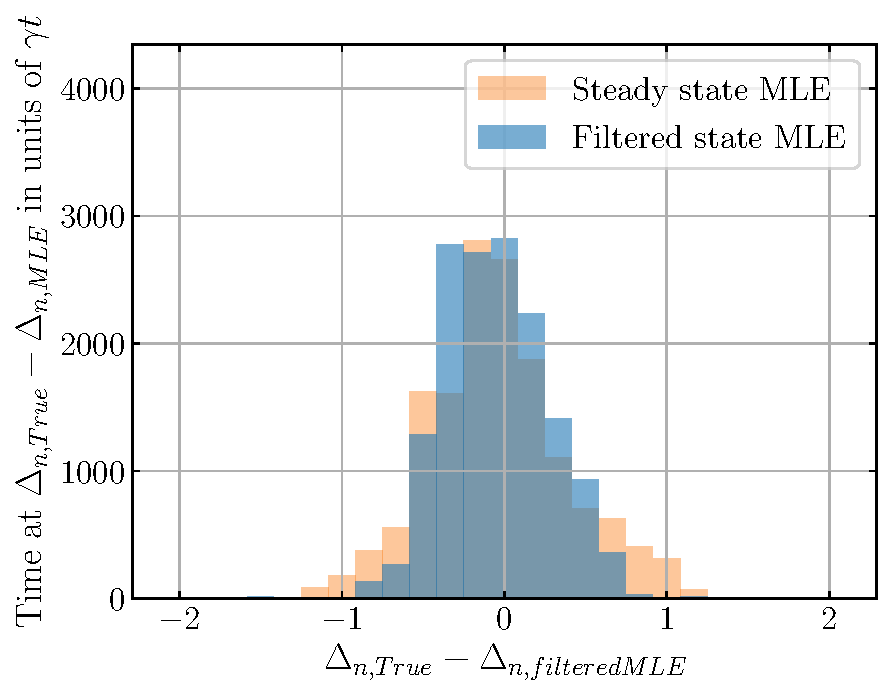
\includegraphics[width=0.4\textwidth]{forward_histogram.pdf}
%    \caption{The histogram of $B_{true}(t) - ML_{forward}(t)$ binned in time.}
%    \label{forward_histogram}
%\end{figure}
%
%\begin{figure}
%    \centering
%    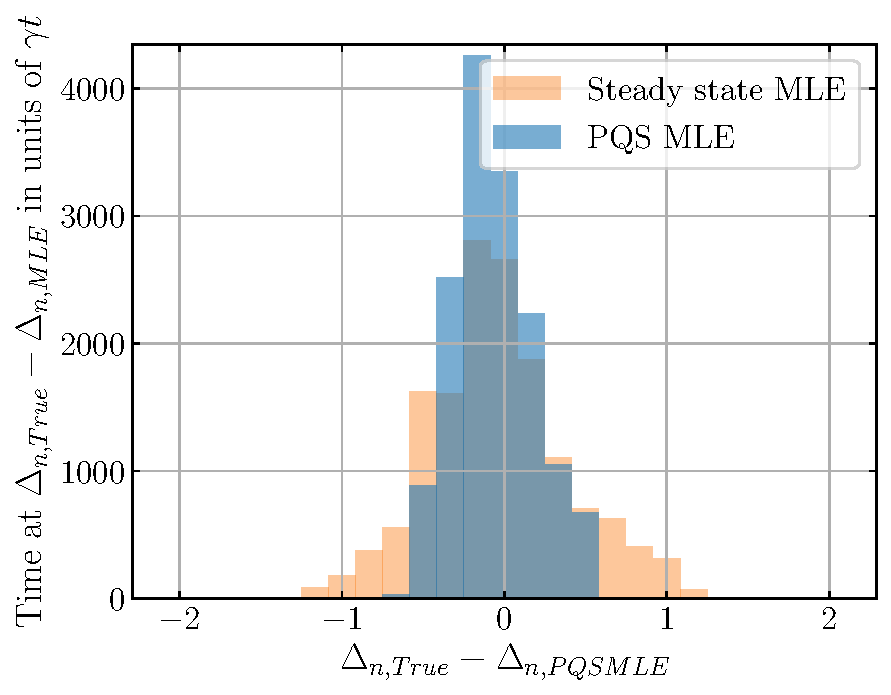
\includegraphics[width=0.4\textwidth]{PQS_histogram.pdf}
%    \caption{The histogram of $B_{true}(t) - ML_{PQS}(t)$ binned in time.}
%    \label{PQS_histogram}
%\end{figure}
%
%\subsubsection{Autocorrelation function}
%The machinery for calculating autocorrelations of $B_{true}$ and $ML{PQS}$ functions for a single run or averaging over a number of runs has been made. For the run used for this short resumé paper the autocorrelations are shown in figure \ref{autocorrelations}. Since the Ehrenfest Dog-Flea model is a discrete rate system converging to the Ornstein-Uhlenbeck function for discretization steps going to zero in both space (B-field here) and time, the Dog-Flea model should have a similar autocorrelation function. This is known to be a function of the form (from Lia's thesis)
%\begin{equation}
%C_{W(t)W(t+\tau)}=\sqrt{\frac{1}{1+\tau/t}}.
%\end{equation}
%Thus a formal comparison should be easily possible, but has not been implemented as of yet.
%\begin{figure}
%    \centering
%    \includegraphics[width=0.4\textwidth]{autocorrelation.pdf}
%    \caption{Autocorrelation functions of $B_{true}$ and $B_{i}$.}
%    \label{autocorrelations}
%\end{figure}


\section{Conclusion}



\begin{thebibliography}{10}
\expandafter\ifx\csname natexlab\endcsname\relax\def\natexlab#1{#1}\fi
\expandafter\ifx\csname bibnamefont\endcsname\relax
  \def\bibnamefont#1{#1}\fi
\expandafter\ifx\csname bibfnamefont\endcsname\relax
  \def\bibfnamefont#1{#1}\fi
\expandafter\ifx\csname citenamefont\endcsname\relax
  \def\citenamefont#1{#1}\fi
\expandafter\ifx\csname url\endcsname\relax
  \def\url#1{\texttt{#1}}\fi
\expandafter\ifx\csname urlprefix\endcsname\relax\def\urlprefix{URL }\fi
\providecommand{\bibinfo}[2]{#2}
\providecommand{\eprint}[2][]{\url{#2}}



%% En sublim kilde til den generaliserede Ehrenfestmodel
\bibitem{hauert2004dogs}
	Hauert, Ch and Nagler, Jan and Schuster, Heinz Georg, Journal of statistical physics, volume 116m,  number 5-6, pages 1453--1469, (2004)



\end{thebibliography}


\end{document}
